\documentclass{report}

%% Don't import the header multiple times

\ifdefined\HEADERIMPORTED
\else
\newcommand\HEADERIMPORTED[0]{This file is HEADERIMPORTED}
\usepackage{amssymb}

\usepackage{amsmath}


% For typesetting tree rules
\usepackage{mathpartir}

% For colouring code
\usepackage{xcolor}


\usepackage{array}   % for \newcolumntype macro
\usepackage{tikz-cd}
\usepackage{tabstackengine}
\usepackage{breqn}
\usepackage{stmaryrd}

\usepackage{float} % extra options for figure placement

% For drawing boxed
\usepackage{framed}

% for code fragments + highlighting
\usepackage{listings}

% For roman numerals
\usepackage{enumitem}


\usepackage{amsthm}
%Theorems
\usepackage[utf8]{inputenc}
\usepackage[english]{babel}

\ifdefined\PRESENTATIONMODE
\else
\usepackage[a4paper,includeheadfoot,margin=2.54cm]{geometry}
\newtheorem{theorem}{Theorem}[section]
\newtheorem{corollary}{Corollary}[theorem]
\newtheorem{lemma}[theorem]{Lemma}
\newtheorem{definition}{Definition}[section]

\newtheorem{aside}{Aside}[section]
\newtheorem{property}[theorem]{Property}
\theoremstyle{definition}
\fi



\usepackage{tikz}

\definecolor{grey}{rgb}{0.75, 0.75, 0.75}
\definecolor{DarkGreen}{rgb}{0.1, 0.6, 0.1}

\usetikzlibrary{shapes.geometric,fit}
\usetikzlibrary{arrows,automata,positioning}
\usetikzlibrary{decorations.pathreplacing,calc}



\setstackEOL{\cr}
\setstackgap{L}{\normalbaselineskip}

\newcommand\todo[1]{\textbf{TODO: #1}}
\newcommand\needsRef[1]{\textbf{Reference Needed: (#1)}}
\newcommand\fixLayout[1]{\textbf{Fix Layout: #1}}


%% Rule Names
% Prefixes
\newcommand{\tprefix}[0]{T-}
\newcommand{\eprefix}[0]{E-}
\newcommand{\sprefix}[0]{S-}
\newcommand\equationalprefix[0]{Eq-}
\newcommand\envprefix[0]{Env-}
\newcommand\pprefix[0]{\eprefix\envprefix}

\newcommand\subprefix[0]{Sb-}
\newcommand\weakenprefix[0]{Wk-}

% Base  rule names
\newcommand\basenil[0]{Nil}
\newcommand\baseextend[0]{Extend}

\newcommand{\baseground}[0]{Ground}
\newcommand{\baseweaken}[0]{Weaken}
\newcommand{\basevar}[0]{Var}
\newcommand\basefn[0]{Fn}
\newcommand\baseeffect[0]{Effect}
\newcommand\basequant[0]{Quantification}


\newcommand\baseunit[0]{Unit}
\newcommand\basetrue[0]{True}
\newcommand\basefalse[0]{False}
\newcommand\baseconst[0]{Const}
\newcommand\basesubtype[0]{Subtype}
\newcommand\basegen[0]{Effect-Gen}
\newcommand\basespec[0]{Effect-Spec}
\newcommand\basereturn[0]{Return}
\newcommand\baseapply[0]{Apply}
\newcommand\baseif[0]{If}
\newcommand\basebind[0]{Bind}

\newcommand\basetransitive[0]{Transitive}
\newcommand\basereflexive[0]{Reflexive}

\newcommand{\baseid}[0]{Id}
\newcommand\baseproject[0]{Project}

% Effect Weakening Rule Names
\newcommand{\eid}[0]{\eprefix\baseid}
\newcommand{\eproject}[0]{\eprefix\baseproject}
\newcommand{\eextend}[0]{\eprefix\baseextend}

% Term Weakening Rule Names
\newcommand{\tid}[0]{\tprefix\baseid}
\newcommand{\tproject}[0]{\tprefix\baseproject}
\newcommand{\textend}[0]{\tprefix\baseextend}

% Effect Substitution Rule Names
\newcommand\esubnil[0]{\eprefix\basenil}
\newcommand\esubextend[0]{\eprefix\baseextend}

% Term Substitution Rule Names

\newcommand\tsubnil[0]{\tprefix\basenil}
\newcommand\tsubextend[0]{\tprefix\baseextend}

% Type environment Rule Names
\newcommand\envnil[0]{\envprefix\basenil}
\newcommand\envextend[0]{\envprefix\baseextend}
% Effect Environment rule names
\newcommand\pnil[0]{\pprefix\basenil}
\newcommand\pextend[0]{\pprefix\baseextend}
% Equational equality rule names
\newcommand{\eqbeta}[0]{\equationalprefix Lambda-Beta}
\newcommand{\eqeta}[0]{\equationalprefix Lambda-Eta}
\newcommand{\eqeffbeta}[0]{\equationalprefix Effect-Beta}
\newcommand{\eqeffeta}[0]{\equationalprefix Effect-Eta}
\newcommand\eqleftunit[0]{\equationalprefix Left-Unit}
\newcommand\eqrightunit[0]{\equationalprefix Right-Unit}
\newcommand\equnitequiv[0]{\equationalprefix Unit}
\newcommand\eqiftrue[0]{\equationalprefix If-True}
\newcommand\eqiffalse[0]{\equationalprefix If-False}
\newcommand\eqifeta[0]{\equationalprefix If-Eta}
\newcommand\eqassociativity[0]{\equationalprefix Associativity}

\newcommand{\eqreflexive}[0]{\equationalprefix\basereflexive}
\newcommand\eqtransitive[0]{\equationalprefix\basetransitive}
\newcommand\eqsymmetric[0]{\equationalprefix Symmetric}

\newcommand\equnit[0]{\equationalprefix\baseunit}
\newcommand\eqtrue[0]{\equationalprefix\basetrue}
\newcommand\eqfalse[0]{\equationalprefix\basefalse}
\newcommand\eqconst[0]{\equationalprefix\baseconst}
\newcommand{\eqvar}[0]{\equationalprefix\basevar}
\newcommand\eqweaken[0]{\equationalprefix\baseweaken}
\newcommand\eqfun[0]{\equationalprefix\basefn}
\newcommand\eqsubtype[0]{\equationalprefix\basesubtype}
\newcommand\eqgen[0]{\equationalprefix\basegen}
\newcommand\eqspec[0]{\equationalprefix\basespec}
\newcommand\eqreturn[0]{\equationalprefix\basereturn}
\newcommand\eqapply[0]{\equationalprefix\baseapply}
\newcommand\eqif[0]{\equationalprefix\baseif}
\newcommand\eqbind[0]{\equationalprefix\basebind}

% Term rule names
\newcommand\vunit[0]{\baseunit}
\newcommand\vtrue[0]{\basetrue}
\newcommand\vfalse[0]{\basefalse}
\newcommand\vconst[0]{\baseconst}
\newcommand{\vvar}[0]{\basevar}
\newcommand\vweaken[0]{\baseweaken}
\newcommand\vfun[0]{\basefn}
\newcommand\vsubtype[0]{\basesubtype}
\newcommand\vgen[0]{\basegen}
\newcommand\vspec[0]{\basespec}
\newcommand\vreturn[0]{\basereturn}
\newcommand\vapply[0]{\baseapply}
\newcommand\vif[0]{\baseif}
\newcommand\vbind[0]{\basebind}

%Effect rule names
\newcommand\eground[0]{\eprefix\baseground}
\newcommand\evar[0]{\eprefix\basevar}
\newcommand\eweaken[0]{\eprefix\baseweaken}
\newcommand\ecompose[0]{\eprefix Compose}

% Type rule names
\newcommand{\tground}[0]{\tprefix\baseground}
\newcommand{\tfun}[0]{\tprefix\basefn}
\newcommand{\teffect}[0]{\tprefix\baseeffect}
\newcommand{\tquant}[0]{\tprefix\basequant}

% Subtyping rule names
\newcommand{\stransitive}[0]{\sprefix\basetransitive}
\newcommand{\sreflexive}[0]{\sprefix\basereflexive}
\newcommand{\sground}[0]{\sprefix\baseground}
\newcommand{\sfun}[0]{\sprefix\basefn}
\newcommand{\seffect}[0]{\sprefix\baseeffect}
\newcommand{\squant}[0]{\sprefix\basequant}


\newcommand{\s}{\;}
\newcommand{\doin}[3]{\texttt{do}\s #1 \leftarrow #2 \s\texttt{in}\s #3\s}
\newcommand\apply[2]{#1\s#2}
\newcommand{\pifthenelse}[4]{\texttt{if}_{\textcolor{purple}{#1}}\s#2\s \texttt{then}\s #3 \s\texttt{else} \s#4\s}
\newcommand\ifthenelse[5]{\pifthenelse{#1, #2}{#3}{#4}{#5}}
\newcommand\const[1]{\texttt{k}^{\color{purple} #1}}
\newcommand\return[1]{\texttt{return} \s#1\s}


\newcommand\lam[3]{\lambda #1 \colon {\color{purple}#2}. #3\s}
\renewcommand\u[0]{\texttt{()}}
\newcommand{\U}[0]{\texttt{Unit}}
\renewcommand\t[0]{\texttt{true}}
\newcommand\f[0]{\texttt{false}}
\newcommand{\B}[0]{\texttt{Bool}}
\newcommand{\G}[0]{\Gamma}
\newcommand\D{\Delta}


% draw type relations
\newcommand{\typerelation}[3]{{\color{DarkGreen}#1} \vdash #2 \colon {\color{blue}#3}}
\newcommand\wellformed[2]{{\color{DarkGreen}#1}\vdash {\color{blue}#2}}
\newcommand\wellformedok[2]{\ok{{\color{DarkGreen}#1}\vdash {\color{blue} #2}}}

\newcommand{\wellformedtype}[2]{\typerelation{#1}{#2}{\type}}
\newcommand{\wellformedeffect}[2]{\typerelation{#1}{#2}{\effect}}
\newcommand{\wellformedF}[2]{\typerelation{#1}{#2}{F}}



\newcommand{\gtyperelation}[2]{\typerelation{\G}{#1}{#2}}
 

\newcommand\treerulez[1]{\inferrule{ }{#1}}
\newcommand\treeruleI[2]{\inferrule{#1}{#2}}
\newcommand\treeruleII[3]{\inferrule{#1 \\ #2}{#3}}
\newcommand\treeruleIII[4]{\inferrule{#1 \\ #2 \\ #3}{#4}}
\newcommand\treeruleIV[5]{\inferrule{#1 \\ #2 \\ #3 \\ #4}{#5}}
\newcommand\treeruleV[6]{\inferrule{#1 \\ #2 \\ #3 \\ #4 \\ #5}{#6}}

\newcommand\ntreerulez[2]{(\text{#1})\inferrule{ }{#2}}
\newcommand\ntreeruleI[3]{(\text{#1})\inferrule{#2}{#3}}
\newcommand\ntreeruleII[4]{(\text{#1})\inferrule{#2 \\ #3}{#4}}
\newcommand\ntreeruleIII[5]{(\text{#1})\inferrule{#2 \\ #3 \\ #4}{#5}}
\newcommand\ntreeruleIV[6]{(\text{#1})\inferrule{#2 \\ #3 \\ #4 \\ #5}{#6}}
\newcommand\ntreeruleV[7]{(\text{#1})\inferrule{#2 \\ #3 \\ #4 \\ #5 \\ #6}{#7}}

\newcommand\condtreerulez[3]{(\text{#1})\inferrule{ }{#2}(\text{if } #3)}
\newcommand\condtreeruleI[4]{(\text{#1})\inferrule{#2}{#3}(\text{if } #4)}
\newcommand\condtreeruleII[5]{(\text{#1})\inferrule{#2 \\ #3}{#4}(\text{if } #5)}
\newcommand\condtreeruleIII[6]{(\text{#1})\inferrule{#2 \\ #3 \\ #4}{#5}(\text{if } #6)}
\newcommand\condtreeruleIV[7]{(\text{#1})\inferrule{#2 \\ #3 \\ #4 \\ #5}{#6}(\text{if } #7)}
\newcommand\condtreeruleV[8]{(\text{#1})\inferrule{ #2 \\ #3 \\ #4 \\ #5 \\ #6 }{#7}(\text{if } #8)}



\newcommand{\subtype}[0]{\leq\colon}
\newcommand\subeffect[0]{\leq}

\newcommand{\M}[2]{\texttt{M}_{#1}{#2}}

\newcommand\lamtype[3]{#1 \rightarrow \M{#2}{#3}}
\newcommand{\1}[0]{\texttt{1}}

\newcommand\e[0]{\epsilon}

\newcommand{\db}[1]{{\bf [\![}#1{\bf ]\!]}}
\newcommand{\deno}[1]{\db{#1}}
\newcommand\after\circ
\newcommand\term[1]{\langle\rangle_{#1}}

\newcommand\bindmu[0]{\mu}
\newcommand\point[1]{\eta_{#1}}
\newcommand\bind[3]{\bindmu_{#1, #2, #3}}

\newcommand\T[2]{T_{#1}{#2}}

\newcommand\pr[2]{\langle#1, #2\rangle}
\newcommand\finpr[2]{\langle #1\rangle_{#2}}

\newcommand\strengtht[0]{\texttt{t}}
% tensor strength Nat-tran
\newcommand\tstrength[3]{\strengtht_{#1, #2, #3}}

% Id morphism
\newcommand\Id[1]{\texttt{Id}_{#1}}

\newcommand\idg[0]{\Id{\G}}
% beta-eta equivalence
\newcommand\beequiv[0]{\approx}
% Substitutions
\newcommand\si{\sigma}

\newcommand{\sub}[1]{[#1]}
\newcommand{\ssub}[2]{[#2 / #1]}
\newcommand{\ssi}[0]{\sub{\si}}

% beta-eta equivalence relation
\newcommand{\berelation}[4]{\typerelation{#1}{#2 \beequiv #3}{#4}}
\newcommand{\gberelation}[3]{\gtyperelation{#1 \beequiv #2}{#3}}


% Shortcuts for denotational equality
\newcommand{\denoequality}[4]{\deno{\typerelation{#1}{#2}{#4}} = \deno{\typerelation{#1}{#3}{#4}}}
\newcommand{\gdenoequality}[3]{\denoequality{\G}{#1}{#2}{#3}}

% Shorthand for monad types
\newcommand\mea[0]{\M{\e}{A}}
\newcommand\meb[0]{\M{\e}{B}}
\newcommand\mec[0]{\M{\e}{C}}

\newcommand\tea[0]{\T{\e}{A}}
\newcommand\teb[0]{\T{\e}{B}}
\newcommand\tec[0]{\T{\e}{C}}


\newcommand\moa[0]{\M{\1}{A}}
\newcommand\mob[0]{\M{\1}{B}}
\newcommand\moc[0]{\M{\1}{C}}

\newcommand\toa[0]{\T{\1}{A}}
\newcommand\tob[0]{\T{\1}{B}}
\newcommand\toc[0]{\T{\1}{C}}

\newcommand\aeb[0]{\lamtype{A}{\e}{B}}

% Shorthand for Gammas
\newcommand{\gax}[0]{\G, x\colon A}
\newcommand{\gby}[0]{\G, y\colon B}

% reduction function
\newcommand{\reduce}[0]{reduce}



% Combinators for building delta-based tree proof terms
\newcommand{\deltavrule}[4]{
    \ntreeruleII{\vsubtype}{\treeruleI{\D}{\typerelation{#1}{#2}{#3}}}{#3 \subtype #4}{\typerelation{#1}{#2}{#4}}}

\newcommand{\deltavruleprime}[4]{
    \ntreeruleII{\vsubtype}{\treeruleI{\D'}{\typerelation{#1}{#2}{#3}}}{#3 \subtype #4}{\typerelation{#1}{#2}{#4}}}

\newcommand{\deltavruleprimeprime}[4]{
        \ntreeruleII{\vsubtype}{\treeruleI{\D'}{\typerelation{#1}{#2}{#3}}}{#3 \subtype #4}{\typerelation{#1}{#2}{#4}}}
    
\newcommand{\deltacrule}[6]{
            \ntreeruleII{Subeffect}{\treeruleI{\D}{\typerelation{#1}{#2}{\M{#3}{#4}}}}{\subeffecttree{#3}{#4}{#5}{#6}}{\typerelation{#1}{#2}{\M{#5}{#6}}}}
\newcommand{\deltacruleprime}[6]{
    \ntreeruleII{Subeffect}{\treeruleI{\D'}{\typerelation{#1}{#2}{\M{#3}{#4}}}}{
    \subeffecttree{#3}{#4}{#5}{#6}}{\typerelation{#1}{#2}{\M{#5}{#6}}}}
\newcommand{\deltacruleprimeprime}[6]{
    \ntreeruleII{\vsubtype}{\treeruleI{\D''}{\typerelation{#1}{#2}{\M{#3}{#4}}}}{
        \subeffecttree{#3}{#4}{#5}{#6}}{\typerelation{#1}{#2}{\M{#5}{#6}}}}
                            

\newcommand{\p}[0]{\pi_1}
\newcommand{\pp}[0]{\pi_2}

% short-hands for weakening
\newcommand{\wrel}[3]{#1 \colon {\color{blue}#2} \triangleright {\color {blue} #3}}
\newcommand{\ok}[1]{{\color{blue} #1} \texttt{ Ok}}
\newcommand\okt[0]{\texttt{Ok}}
\renewcommand\i[0]{\iota}
\newcommand\w{\omega}
\newcommand\dom[1]{\texttt{dom}(#1)}
\newcommand\x{\times}


\newcommand\fev[1]{fev(#1)}
\newcommand\union[0]{\cup}


% Combinators to build tree proofs
\newcommand{\truleconst}[0]{\ntreeruleI{\vconst}{\ok{\G}}{\gtyperelation{\const{A}}{A}}}
\newcommand{\truleunit}[0]{\ntreeruleI{\vunit}{\ok{\G}}{\typerelation{\G}{\u}{\U}}}
\newcommand{\truletrue}[0]{\ntreeruleI{\vtrue}{\ok{\G}}{\typerelation{\G}{\t}{\B}}}
\newcommand{\trulefalse}[0]{\ntreeruleI{\vfalse}{\ok{\G}}{\typerelation{\G}{\f}{\B}}}


\newcommand{\E}[0]{\mathbb{E}}
\renewcommand{\dot}{\cdot}
\newcommand{\gens}[0]{\colon\colon=}
\newcommand{\nil}[0]{\diamond}
\newcommand{\ground}[0]{\gamma}

% Terminal object of C
\newcommand{\terminal}[0]{\texttt{\1}}

% The category C
\newcommand{\C}[0]{\mathbb{C}}
\newcommand{\Cz}[0]{\C_0}
\newcommand\DC[0]{\mathbb{D}}

% The category of locally-small categories
\newcommand{\Cat}[0]{\texttt{Cat}}
% Sub-effect Nat-trans
\newcommand{\dse}[2]{\db{#1 \subeffect #2}}

\newcommand\app[0]{\texttt{app}}
\newcommand\cur[1]{\texttt{cur}(#1)}
\newcommand{\ifnt}[1]{\texttt{If}_{#1}}


\newcommand{\setto}{\colon=}
\newcommand{\fv}[1]{\texttt{fv}(#1)}

% shorthand for inserting text to equations
\newcommand\qt[1]{\quad\text{#1}}

% Co-product short-hands
\newcommand\inr[0]{\texttt{inr}}
\newcommand\inl[0]{\texttt{inl}}
    
\newcommand\fld[2]{[#1,#2]}
\newcommand{\diag}[1]{\delta_{#1}}
\newcommand{\twist}[2]{\tau_{#1, #2}}

\newcommand\ifMorph[3]{\app\after((\fld{\cur{#2\after\pp}}{\cur{#3\after\pp}}\after #1)\times \idg)\after \diag{\G}}


% Polymorphic short-hands
\newcommand\elam[2]{\Lambda #1. #2}
\newcommand{\eapp}[2]{#1\s#2}
\renewcommand{\a}[0]{\alpha}
\newcommand{\all}[2]{\forall #1. #2}
\renewcommand{\P}[0]{\Phi}

\renewcommand{\b}[0]{\beta}
\newcommand{\g}[0]{\gamma}
\renewcommand\d[0]{\delta}
\newcommand\oke[2]{\wellformedok{#1}{#2}}
\newcommand\etyperelation[4]{\typerelation{#1\mid#2}{#3}{#4}}
\newcommand{\gpetyperelation}[2]{\etyperelation{\P}{\G}{#1}{#2}}
\newcommand{\gppetyperelation}[2]{\etyperelation{\P'}{\G}{#1}{#2}}


\newcommand{\eberelation}[5]{\berelation{#1\mid#2}{#3}{#4}{#5}}
\newcommand{\gpeberelation}[3]{\berelation{\P\mid\G}{#1}{#2}{#3}}
\newcommand{\gppeberelation}[3]{\berelation{\P'\mid\G}{#1}{#2}{#3}}

\newcommand{\dotp}[0]{\dot_\P}
\newcommand{\fntype}[2]{#1\rightarrow #2}
\newcommand{\ab}[0]{\fntype{A}{B}}

\newcommand\wrelw[2]{\wrel{\w}{#1}{#2}}
\renewcommand\proof[0]{\paragraph{Proof:}}
\newcommand{\case}[1]{\paragraph{Case #1:}}
\newcommand{\subcase}[1]{\subparagraph{Case: #1}}
\newcommand\bi[0]{By inversion}

%pre-filled effect-weakening relations
\newcommand\ewrel[4]{\wellformed{#1}{\color{black}\wrel{#2}{#3}{#4}}}
\newcommand\pewrel[3]{\ewrel{\P}{#1}{#2}#3}
\newcommand\ppewrel[3]{\ewrel{\P'}{#1}{#2}#3}

\newcommand\subtypep[0]{\subtype_\P}
\newcommand\subtypepp[0]{\subtype_{\P'}}
\newcommand\subeffectp[0]{\subeffect_{\P}}
\newcommand\subeffectpp[0]{\subeffect_{\P'}}
\newcommand\subeffectn[0]{\subeffect_{n}}
\newcommand\subeffectz[0]{\subeffect_{0}}

\newcommand{\allI}[0]{\forall_I}
\newcommand{\allII}[0]{\forall_{I'}}
\newcommand\allIU[0]{\forall_{I\times U}}
\newcommand\type[0]{\texttt{Type}}
\newcommand\effect[0]{\texttt{Effect}}
\newcommand\ciw[0]{\C(I, W)}
\newcommand\ciu[0]{\C(I, U)}
\newcommand\ciuw[0]{\C(I\times U, W)}
\newcommand\cipw[0]{\C(I', W)}
\newcommand\cipu[0]{\C(I', U)}
\newcommand\ciuu[0]{\C(I\times U, U)}
\newcommand\cii[0]{\C(I', I)}
\newcommand\Eff[0]{\texttt{Eff}}
\newcommand\Mul[0]{\texttt{Mul}}
\newcommand\singleton[0]{\ast}
\renewcommand\star[0]{^*}
\renewcommand\bar[1]{\overline{#1}}

\newcommand\subtypeg[0]{\subtype_\g}
\newcommand\subtypepa[0]{\subtype_{\P, \a}}
\newcommand\subtypeppa[0]{\subtype_{\P', \a}}

\newcommand\subtypez[0]{\subtype_{0}}
\newcommand\subtypen[0]{\subtype_{n}}

\usepackage{scalerel,stackengine}
\stackMath
\renewcommand\widehat[1]{%
\savestack{\tmpbox}{\stretchto{%
  \scaleto{%
    \scalerel*[\widthof{\ensuremath{#1}}]{\kern.1pt\mathchar"0362\kern.1pt}%
    {\rule{0ex}{\textheight}}%WIDTH-LIMITED CIRCUMFLEX
  }{\textheight}% 
}{2.4ex}}%
\stackon[-6.9pt]{#1}{\tmpbox}%
}
\parskip 1ex

\newcommand\pstar[0]{\p\star}

\newcommand\edeltavrule[5]{\deltavrule{#1 \mid #2}{#3}{#4}{#5}}

\newcommand\subeffecttreep[4]{\ntreeruleII{\teffect}{
    #1\subeffectp #3}{#2 \subtypep #4
}{\M{#1}{
    #2
}\subtypep\M{#3}{#4}}}
\newcommand\subeffecttree[4]{\ntreeruleII{\teffect}{
    #1\subeffect #3}{#2 \subtype #4
}{\M{#1}{
    #2
}\subtype\M{#3}{#4}}}


\newcommand{\edeltavruleprime}[5]{
        \deltavruleprime{#1\mid #2}{#3}{#4}{#5}}
    
\newcommand{\edeltavruleprimeprime}[5]{
        \deltavruleprimeprime{#1\mid #2}{#3}{#4}{#5}}
    
\newcommand{\edeltacrule}[6]{
            \ntreeruleII{\vsubtype}{
                \treeruleI{
                    \D
                }{
                    \typerelation{\P\mid#1}{#2}{\M{#3}{#4}}
                }
            }{
                \ntreeruleII{\teffect}{
                    #4 \subtypep #6
                    }{
                         #3 \subeffectp #5
                }{
                    \M{#3}{#4}\subtypep{\M{#5}{#6}}
                }
            }{
                \typerelation{\P\mid #1}{#2}{\M{#5}{#6}}
            }
        }
        

        \newcommand{\edeltacruleprime}[6]{
            \ntreeruleII{\vsubtype}{
                \treeruleI{
                    \D'
                }{
                    \typerelation{\P\mid #1}{#2}{\M{#3}{#4}}
                }
            }{
                \ntreeruleII{\teffect}{
                    #4 \subtypep #6
                }{#3 \subeffectp #5
                }{
                    \M{#3}{#4}\subtypep{\M{#5}{#6}}
                }
            }{
                \typerelation{\P\mid #1}{#2}{\M{#5}{#6}}
            }
        }
                   

        \newcommand{\edeltacruleprimeprime}[6]{
            \ntreeruleII{\vsubtype}{
                \treeruleI{
                    \D''
                }{
                    \typerelation{\P\mid #1}{#2}{\M{#3}{#4}}
                }
            }{
                \ntreeruleII{\teffect}{
                    #4 \subtypep #6
                    }{ #3 \subeffectp #5
                }{
                    \M{#3}{#4}\subtypep{\M{#5}{#6}}
                }
            }{
                \typerelation{\P\mid #1}{#2}{\M{#5}{#6}}
            }
        }

        \newcommand\obj[0]{\texttt{obj }}


        \newcommand{\Tz}[2]{\texttt{T}^0_{#1}#2}
        \newcommand{\Tn}[2]{\texttt{T}^n_{#1}#2}
        \newcommand{\Tm}[2]{\texttt{T}^m_{#1}#2}
        
        \newcommand{\pointz}[1]{\point{#1}^0}
        \newcommand{\pointn}[1]{\point{#1}^n}
        \newcommand{\pointm}[1]{\point{#1}^m}
        
        \newcommand{\bindz}[3]{\bind{#1}{#2}{#3}^0}
        \newcommand{\bindn}[3]{\bind{#1}{#2}{#3}^n}
        \newcommand{\bindm}[3]{\bind{#1}{#2}{#3}^m}
        
        \newcommand\tstrengthz[3]{\tstrength{#1}{#2}{#3}^0}
        \newcommand\tstrengthn[3]{\tstrength{#1}{#2}{#3}^n}
        \newcommand\tstrengthm[3]{\tstrength{#1}{#2}{#3}^m}
        
        \newcommand\set[0]{\texttt{Set}}
        \newcommand\cccat[0]{\textit{CCCat}}

        \newcommand\ev[0]{\vec{\e}}
        \newcommand\emv[0]{\vec{\e_m}}
        \newcommand\env[0]{\vec{\e_n}}
        
        \newcommand\subeffectm[0]{\subeffect_m}
        
        \newcommand\dsem[2]{\db{#1 \subeffectm #2}}
        \newcommand\dsen[2]{\db{#1 \subeffectn #2}}
        \newcommand\dsez[2]{\db{#1 \subeffectz #2}}
        \newcommand\dsep[2]{\db{#1 \subeffectp #2}}
        \newcommand\dsepp[2]{\db{#1 \subeffectpp #2}}
        
        \newcommand\allEn[0]{\forall_{E^n}}
        \newcommand\allEm[0]{\forall_{E^m}}
        
        \newcommand\counit[1]{\boldsymbol{\epsilon}_{#1}}
        \newcommand\unit[1]{\boldsymbol{\eta}_{#1}}


        
%% Adequacy shorthands
\newcommand{\relates}[0]{\lhd}
\newcommand{\logRel}[3]{#1 \relates_{#2} #3}
\newcommand{\plogRel}[4]{#1 \relates_{\wellformed{#2}{#3}} #4}

\newcommand{\zberelation}[3]{\berelation{}{#1}{#2}{#3}}
\newcommand\ztyperelation[2]{\typerelation{}{#1}{#2}}

\newcommand{\N}[0]{\mathbb{N}}
\renewcommand\put[0]{\texttt{put}}
\newcommand\ecput[0]{\texttt{EC}_\put}
\newcommand\ecputA[0]{\texttt{EC}_\put^A}
\newcommand\ecputG[0]{\texttt{EC}_\put^G}

\newcommand\mna[0]{\M{n}{A}}
\newcommand\mmb[0]{\M{m}{B}}
\newcommand\mnb[0]{\M{n}{B}}
\newcommand\mma[0]{\M{m}{A}}

\newcommand{\setcomp}[2]{\{#1 \mid #2 \}}
\fi


% Appendix document proving the S-category properties of the functor categories [E^n, \Set]

\begin{document}
\section{Base Category is Monoidal}

We construct the base category, $\Eff$, as follows:

\begin{itemize}
    \item $U = E$, the set of ground effects in the non-polymorphic language.
    \item $\1$ is a singleton set.
    \item $U^n = E^n$, set of $n$-wide tuples of effects, $\vec{\e}$
\end{itemize}

Hence when we treat effects that are well formed in $\P$ as morphisms, $E^n \rightarrow E$ in $\Eff$, we should treat them as functions $f: E^n \rightarrow E$. Ground effects become point functions: $e: \1 \rightarrow E$, so the denotation of a ground effect is the constant value function: $\deno{\typerelation{\P}{e}{\effect}} = \ev \mapsto e$. We extend the multiplication of ground effects to multiplication on effect functions, giving us our $\Mul_n$ operation $\Mul_n(f, g)(\ev) = (f\ev)\dot(g\ev)$. This $\Mul_n$ satisfies the naturality and monoidal requirements, as seen in figure \ref{MulMonoidAndNatural}. It is also trivially the case that $\Mul_n(\deno{\typerelation{\P}{e_1}{\effect}}, \deno{\typerelation{\P}{e_2}{\effect}}) = \deno{\typerelation{\P}{e_1\dot e_2}{\effect}}$.

\begin{figure}
    \begin{framed}
        \begin{framed}
            \centering\textbf{Naturality} 
            \begin{equation*}
                (\Mul_m(f, g)\after \theta)\ev = (f(\theta\ev))\dot(g(\theta\ev)) = (\Mul_n(f\after\theta), (g\after\theta))\ev
            \end{equation*}
        \end{framed} 
        
        \begin{framed}
            \centering\textbf{Left and Right Identity}
            \begin{minipage}{.45\textwidth}
                \begin{align*}
                    \Mul_n(\deno{\typerelation{\P}{\1}{\effect}}, f)(\ev) & = (\1\ev)\dot(f\ev)\\
                    & = (\1)\dot(f\ev)\\
                    & = f\ev\\
                \end{align*}
            \end{minipage}
            \quad
            \begin{minipage}{.45\textwidth}
                \begin{align*}
                    \Mul_n(f, \deno{\typerelation{\P}{\1}{\effect}})(\ev) & = (f\ev)\dot(\1\ev)\\
                    & = (f\ev)\dot(\1)\\
                    & = f\ev\\
                \end{align*}
            \end{minipage}
        \end{framed}

        \begin{framed}
            \centering\textbf{Monoid Associativity}

            \begin{align*}
                \Mul_n(f, \Mul_n(g, h))(\ev) & = (f\ev)\dot((g\ev)\dot(h\ev))\\
                & = ((f\ev)\dot(g\ev))\dot(h\ev)\\
                & = \Mul_n(\Mul_n(f,g), h)(\ev)
            \end{align*}
        \end{framed}
    \end{framed}
    
    
    \caption{Our pick for $\Mul$ is natural and is a monoid at each $n$.}
    \label{MulMonoidAndNatural}
\end{figure}

\section{S-Categories}
The semantic category, $[E^0, \set]$ of the effect-environment $\nil$ is isomorphic to $\set$. Since each effect-environment is alpha equivalent to a natural number, the semantic category for $\P$ shall be represented as $\C(\P) = \C(n) = [E^n, \set]$, the category of functions $E^n\rightarrow \set$. Objects in $[E^n, \set]$ are functions and we describe them by their actions on a generic vector of ground effects, $\ev$. Morphisms in $[E^n, \set]$ are natural transformations between the functions. So:

\begin{align*}
    m:\quad&A \rightarrow B \qt{ In $[E^n, \set]$}\\
    m\ev:\quad& A\ev \rightarrow B\ev \qt{In $\set$}\\
    (f\after g)\ev =\quad& (f\ev)\after(g\ev)\\
    \Id{A}(\ev) =\quad& \Id{A\ev}
\end{align*}

So morphisms are dependently typed functions from a vector of ground effects to morphisms in $\set$.
\subsection{Each S-Category is a CCC}
Since $\set$ is complete and a CCC, and $E^n$ is small, since $E$ is small, $[E^n, \set]$ is a CCC.

\begin{align*}
    (A\times B)\ev & = (A\ev)\times(B\ev)\\
    \1\ev & = \1\\
    (B^A)\ev &= (B\ev)^{(A\ev)}\\
    \p\ev & = \p\\
    \pp\ev & = \pp\\
    \app\ev & = \app\\
    \cur{f}\ev & = \cur{f\ev}\\
    \pr{f}{g}\ev & = \pr{f\ev}{g\ev}\\
\end{align*}

\subsection{The Terminal Co-Product}

We can define the co-product point-wise.

\begin{align*}
    (\1 + \1)\ev & = (\1\ev + \1\ev)\\
    & = (\1 + \1)\\
    \inl\ev &= \inl\\
    \inr\ev &= \inr\\
    [f, g]\ev &= [f\ev, g\ev]\\
\end{align*}

This preserves the co-product diagram.

\begin{align*}
    ([f, g]\after\inl)\ev & = [f\ev, g\ev]\after \inl\\
    & = f\ev\\
    & \square\\
    ([f, g]\after\inr)\ev& = [f\ev, g\ev]\after \inr\\
    & = f\ev\\
    & \square\\
\end{align*}

$[f, g]$ is also unique in $[E^n, \set]$. Suppose $l \after \inl = f$ and $l\after \inr = g$ in $[E^n, \set]$. Then $l\ev \after \inl = f\ev$ and $l\ev \after\inr = g\ev$. Hence by the co-product in $\set$, $l = [f\ev, g\ev]$ so $l = [f, g]$.


\subsection{Ground Types and Terms}
Each ground type in the non-polymorphic calculus has a fixed denotation $\deno{\g}\in\obj\set$. The ground type in the polymorphic calculus hence has a denotation represented by the constant function.

\begin{align*}
    \deno{\g}:&\quad E^n\rightarrow \obj\set\\
    \ev \mapsto&\quad  \deno{\g}\\
\end{align*}

Each constant term $\const{A}$ in the non-polymorphic calculus has a fixed denotation $\deno{\const{A}}\in\set(\1, A)$. So the morphism $\deno{\const{A}}$ in $[E^n, \set]$ is the corresponding constant dependently typed morphism returning the $\deno{\const{A}}$ function in $\set$.

\begin{align*}
    \deno{\const{A}}:&\quad[E^n, \set](\1, A)\\
    \ev\mapsto&\quad\deno{\const{A}}
\end{align*}

\subsection{Graded Monad}
Given the strong graded monad $(\Tz{}{}, \pointz{}{}{}, \bindmu^0, \strengtht^0)$ on $\set$, we can construct an appropriate graded monad $(\Tn{}{}, \pointn{}{}{}, \bindmu^n,\strengtht^n)$ on $[E^n, \set]$. Through some mechanical proof and the naturality of the $\set$ strong graded monad, these morphisms are natural in their type parameters and form a strong graded monad in $[E^n, \set]$.

\begin{align*}
    \Tn{}{}:&\quad(E^n, \dot, \subeffect_n, \1_n) \rightarrow [[E^n, \set], [E^n, \set]]\\
    (\Tn{f}{A})\ev=&\quad \Tz{(f\ev)}{A\ev}\\
    (\pointn{A})\ev=&\quad\pointz{A\ev}\\
    (\bindn{f}{g}{A})\ev=&\quad\bindz{(f\ev)}{(g\ev)}{(A\ev)}\\
    (\tstrengthn{f}{A}{B})\ev=&\quad\tstrengthz{(f\ev)}{(A\ev)}{(B\ev)}
\end{align*}

\begin{figure}
    \begin{framed}
        \centering\textbf{Naturality of the Graded Monad Transformations}


        \begin{minipage}{.45\textwidth}
            \centering
            \begin{tikzcd}[column sep=huge]
                A\ev 
                \arrow{r}{\pointz{(A\ev)}}
                \arrow{d}{f\ev}
                &
                \Tz{\1}{(A\ev)}
                \arrow{d}{\Tz{\1}{(f\ev)}}
                \\
                B\ev
                \arrow{r}{\pointz{(B\ev)}}
                &
                \Tz{\1}{(B\ev)}
            \end{tikzcd}
        \end{minipage}
        \quad\begin{minipage}{.45\textwidth}
            \centering
            \begin{tikzcd}[column sep=huge]
                \Tz{(f\ev)}{\Tz{(g\ev)}{(A\ev)}}
                \arrow{r}{\bindz{f\ev}{g\ev}{(B\ev)}}
                \arrow{d}{\Tz{f\ev}{\Tz{g\ev}{m\ev}}}
                &
                \Tz{(f\ev)\dot(g\ev)}{(A\ev)}
                \arrow{d}{\Tz{(f\ev)\dot(g\ev)}{m\ev}}
                \\
                \Tz{(f\ev)}{\Tz{(g\ev)}{(B\ev)}}
                \arrow{r}{\bindz{f\ev}{g\ev}{(B\ev)}}
                &
                \Tz{(f\ev)\dot(g\ev)}{(A\ev)}
            \end{tikzcd}
        \end{minipage}
        \\


        
       \begin{minipage}{.45\textwidth}
        \centering
            \begin{tikzcd}[column sep=huge]
                A\ev \times \Tz{f\ev}{(B\ev)}
                \arrow{r}{\tstrengthz{f\ev}{(A\ev)}{(B\ev)}}
                \arrow{d}{(m\ev\times\Id{\Tz{f\ev}{B}})}
                &
                \Tz{f\ev}{(A\ev\times B\ev)}
                \arrow{d}{\Tz{(f\ev)}{(m\ev\times \Id{B\ev})}}
                \\
                A'\ev \times \Tz{f\ev}{(B\ev)}
                \arrow{r}{\tstrengthz{f\ev}{(A'\ev)}{(B\ev)}}
                &
                \Tz{f\ev}{(A'\ev\times B\ev)}
            \end{tikzcd}
        \end{minipage}
        \quad\begin{minipage}{.45\textwidth}
            \centering
            \begin{tikzcd}[column sep=huge]
                A\ev \times \Tz{f\ev}{(B\ev)}
                \arrow{r}{\tstrengthz{f\ev}{(A\ev)}{(B\ev)}}
                \arrow{d}{(\Id{A\ev}\times \Tz{f\ev}{(m\ev)})}
                &
                \Tz{f\ev}{(A\ev\times B\ev)}
                \arrow{d}{\Tz{(f\ev)}{(\Id{A\ev} \times m\ev)}}
                \\
                A\ev \times \Tz{f\ev}{(B'\ev)}
                \arrow{r}{\tstrengthz{f\ev}{(A\ev)}{(B'\ev)}}
                &
                \Tz{f\ev}{(A\ev\times B'\ev)}
            \end{tikzcd}
        \end{minipage}
    \end{framed}
    \caption{Naturality Squares for the graded monad natural transformations. The naturality of each transformation $\a$ in $[E^n, \set]$ derives from the naturality of each of its component transformations $\a\ev$ in $\set$}
    \label{NaturalitySquares}
\end{figure}

\begin{figure}
\begin{framed}
        \centering\textbf{Monad Laws}
    
        \begin{minipage}{.45\textwidth}
            \centering\textbf{Left Unit}
    
    
            \begin{align*}
                (\bindn{\1}{g}{A}\after\pointn{\Tn{f}{A}})\ev &= \bindz{\1}{(f\ev)}{(A\ev)} \after (\pointz{\Tz{f\ev}{A\ev}})\\
                &= \Id{\Tz{f\ev}{A\ev}}\\
                &=(\Id{\Tn{f}{A}})\ev
            \end{align*}
        \end{minipage}\quad
        \begin{minipage}{.45\textwidth}
            \centering\textbf{Right Unit}
    
    
            \begin{align*}
                (\bindn{f}{\1}{A}\after\Tn{f}{\pointn{A}})\ev &= \bindz{(f\ev)}{\1}{(A\ev)} \after \Tz{f\ev}{(\pointz{A\ev})}\\
                &= \Id{\Tz{f\ev}{A\ev}}\\
                &=(\Id{\Tn{f}{A}})\ev
            \end{align*}
        \end{minipage}
        \\
    
        \begin{minipage}{\textwidth}
            \centering\textbf{Monad Associativity} 
    
    
            \begin{align*}
                ((\bindn{f}{(g\dot h)}{A})\after\Tn{f}{(\bindn{g}{h}{A})})\ev &= \bindz{(f\ev)}{((g\ev)\dot(h\ev))}{(A\ev)}\after\Tz{f\ev}{\bindz{(h\ev)}{(g\ev)}{A\ev}}\\
                &= \bindz{((f\ev)\dot(g\ev))}{(h\ev)}{(A\ev)}\after\bindz{(f\ev)}{(g\ev)}{(\Tz{h\ev}{(A\ev)})}\\
                & = (\bindn{f\dot g}{h}{A}\after\bindn{f}{g}{\Tz{h}{A}})\ev
            \end{align*}
        \end{minipage}
\end{framed}
    
    \caption{The monad laws for the graded monad $(\Tn{}{}, \pointn{}{}{}, \bindmu^n,\strengtht^n)$ can be proved component-wise from the graded monad $(\Tz{}{})$ on $\set$.}
    \label{MonadLaws}
\end{figure}

\begin{figure}
\begin{framed}
\centering\textbf{Tensor Strength Laws}

        \begin{framed}
            \centering
            \textbf{Bind Law}
    
            \begin{minipage}{.45\textwidth}
                \centering
                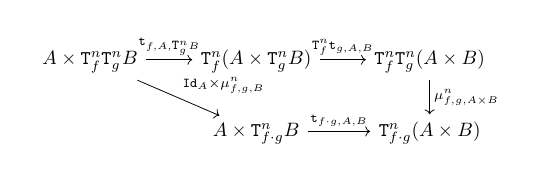
\begin{tikzpicture}[baseline= (a).base]
                    \node[scale=.7] (a) at (0,0){
                \begin{tikzcd}
                    A \times \Tn{f}{\Tn{g}{B}} 
                    \arrow [r, "\tstrength{f}{A}{\Tn{g}{B}}"]
                    \arrow [dr, "\Id{A} \times \bindn{f}{g}{B}"]
                    & 
                    \Tn{f}{(A \times \Tn{g}{B})} 
                    \arrow [r, "\Tn{f}{\tstrength{g}{A}{B}}"]
                    & 
                    \Tn{f}{\Tn{g}{(A \times B)}} 
                    \arrow [d, "\bindn{f}{g}{A \times B}"]
                    \\
                    &
                    A \times \Tn{f \dot g}{B}  
                    \arrow [r, "\tstrength{f \dot g}{A}{B}"] 
                    &
                    \Tn{f \dot g}({A \times B)}
                \end{tikzcd}};
            \end{tikzpicture}
            \end{minipage}
            \quad
            \begin{minipage}{.45\textwidth}
                \centering
                \scalebox{.75}{\parbox{\linewidth}{%
                    \begin{align*}
                        & (\tstrengthn{(f\dot g)}{A}{B}\after (\Id{A}\times \bindn{f}{g}{B}))\ev \\
                        & = (\tstrengthz{((f\ev)\dot (g\ev))}{(A\ev)}{(B\ev)}\after (\Id{A\ev}\times \bindn{(f\ev)}{(g\ev)}{(B\ev)}))\\
                        & = \bindz{(f\ev)}{(g\ev)}{(A\times B)\ev}\after\Tz{f\ev}{(\tstrengthz{(g\ev)}{(A\ev)}{(B\ev)})}\after\tstrengthz{(f\ev)}{(A\ev)}{\Tz{g\ev}{(B\ev)}}\\
                        & = (\bindn{f}{g}{(A\times B)}\after\Tn{f}{(\tstrengthn{g}{A}{B})}\after\tstrengthn{f}{A}{\Tn{g}{(B)}})\ev
                    \end{align*}
                }}
            \end{minipage}
        \end{framed}
    
        \begin{framed}
            \centering
            \textbf{Commutativity with Unit}
    
            \begin{minipage}{.45\textwidth}
                \centering
                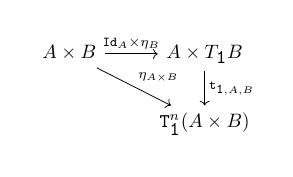
\begin{tikzpicture}[baseline= (a).base]
                    \node[scale=.7] (a) at (0,0){
                
                    \begin{tikzcd}
                        A \times B
                        \arrow [r, "\Id{A} \times \point{B}"]
                        \arrow [rd, "\point{A \times B}"]
                        &
                        A \times \tob 
                        \arrow [d, "\tstrength{\1}{A}{B}"]
                        \\
                        &
                        \Tn{\1}{(A \times B)}
                    \end{tikzcd}
                };
            \end{tikzpicture}
            \end{minipage}
            \quad
            \begin{minipage}{.45\textwidth}
                \centering
                \scalebox{.75}{\parbox{\linewidth}{%
                \begin{align*}
                    (\tstrengthn{\1}{A}{B}\after(\Id{A}\times \pointn{A}))\ev & = \tstrengthz{\1}{(A\ev)}{(B\ev)}\after(\Id{A\ev}\times \pointz{A\ev})\\
                    & = \pointz{A\ev\times B\ev}\\
                    & = (\pointn{A\times B})\ev
                \end{align*}
                }}
            \end{minipage}
        \end{framed}
    
        \begin{framed}
            \centering
            \textbf{Commutativity with $\alpha$}

            Let $\alpha_{A, B, C} = \pr{\p\after\p}{\pr{\pp\after\p}{\pp}}: ((A \times B) \times C) \rightarrow (A \times (B \times C))$
    
    
            \begin{minipage}{.45\textwidth}
                \centering
                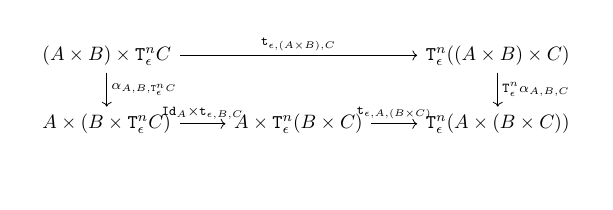
\begin{tikzpicture}[baseline= (a).base]
                    \node[scale=.7] (a) at (0,0){
                    \begin{tikzcd}
                        (A\times B)\times \Tn{\e}{C} 
                        \arrow [rr, "\tstrength{\e}{(A\times B)}{C}"]
                        \arrow [d, "\alpha_{A, B, \Tn{\e}{C}}"]
                        & & \Tn{\e}{((A \times B)\times C)}
                        \arrow [d, "\Tn{\e}{\alpha_{A, B, C}}"]
                        \\
                        A \times (B \times \Tn{\e}{C}) 
                        \arrow [r, "\Id{A}\times\tstrength{\e}{B}{C}"]
                        &
                        A\times\Tn{\e}{(B \times C)} 
                        \arrow [r, "\tstrength{\e}{A}{(B \times C)}"]
                        & \Tn{\e}{(A \times (B \times C))}
                        \\
                    \end{tikzcd}
                };
            \end{tikzpicture}
            \end{minipage}
            \quad
            \begin{minipage}{.45\textwidth}
                \centering
                \scalebox{.75}{\parbox{\linewidth}{%
                \begin{align*}
                    & (\Tn{f}{\alpha_{A, B, C}}\after\tstrengthn{f}{A\times B}{C})\ev \\
                    & = \Tz{f\ev}{\alpha_{A\ev, B\ev, C\ev}} \after\tstrengthz{(f\ev)}{(A\times B)\ev}{(C\ev)}\\
                    & = \tstrengthz{(f\ev)}{(A\ev)}{(B\ev\times C\ev)}\after(\Id{A\ev}\times \tstrengthz{(f\ev)}{(B\ev)}{(C\ev)})\after\alpha_{A\ev, B\ev, C\ev}\\
                    & = (\tstrengthn{f}{A}{(B\times C)}\after(\Id{A}\times \tstrengthn{f}{B}{C})\after\alpha_{A, B, C})\ev\\
                \end{align*}            
                }}
            \end{minipage}
        \end{framed}
\end{framed}

    \caption{The tensor strength laws can be proved component wise from the strength of the monad $\Tz{}{}$}
    \label{TensorStength}
\end{figure}



\subsection{Subeffecting}
Given a collection of subeffecting natural transformation in $\set$, $\deno{\e_1\subeffectz \e_2}: \quad \Tz{\e_1}{} \rightarrow \Tz{\e_2}{}$ we can form subeffect natural transformations in $[E^n, \set]$ as seen in figure \ref{SubEffecting}. This natural transformation has all the required properties. These are proved in figure \ref{SubeffectProperties}.

\begin{figure}
    \begin{framed}
        \centering\textbf{Subeffect Natural Transformation}
    
        \begin{align*}
            \deno{f\subeffectn g}:&\quad\Tn{f}{}\rightarrow \Tn{g}{}\\
            \deno{f\subeffectn g} A \ev:&\quad\Tn{f\ev}{(A\ev)}\rightarrow \Tn{g\ev}{(B\ev)}\\
            =&\quad \deno{f\ev\subeffectz g\ev}A\ev
        \end{align*}
    \end{framed}
    \caption{Definition of subeffecting natural transformations}
    \label{SubEffecting}
\end{figure}

\begin{figure}
    \begin{framed}
        \centering\textbf{Subeffect Natural Transformation Properties}

        \begin{framed}
            \centering
            \textbf{Naturality}
            
            \begin{tikzcd}[column sep=large]
                \Tz{f\ev}{A\ev}
                \arrow{r}{\deno{f\ev\subeffectz g\ev}A\ev}
                \arrow{d}{\Tz{f\ev}{m\ev}}
                &
                \Tz{g\ev}{A\ev}
                \arrow{d}{\Tz{g\ev}{m\ev}}
                \\
                \Tz{f\ev}{B\ev}
                \arrow{r}{\deno{f\ev\subeffectz g\ev}B\ev}
                &
                \Tz{g\ev}{B\ev}
            \end{tikzcd}
        \end{framed}

        \begin{framed}
            \centering
            \textbf{Commutes With Tensor Strength}




    
            \begin{minipage}{.45\textwidth}
                \centering
                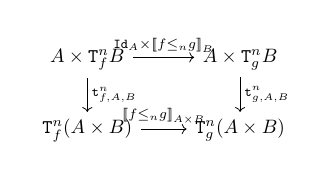
\begin{tikzpicture}[baseline= (a).base]
                    \node[scale=.7] (a) at (0,0){\begin{tikzcd}
                        A \times \Tn{f}{B} \arrow [r, "\Id{A} \times \dsen{f}{g}_B"] \arrow [d, "\tstrengthn{f}{A}{B}"] &
                        A \times \Tn{g}{B} \arrow [d, "\tstrengthn{g}{A}{B}"] \\
                        \Tn{f}{(A \times B)} \arrow [r, "\dsen{f}{g}_{ A \times B}"] &
                        \Tn{g}{(A \times B)} 
                    \end{tikzcd}
                    };
            \end{tikzpicture}
            \end{minipage}
            \quad
            \begin{minipage}{.45\textwidth}
                \centering
                \scalebox{.75}{\parbox{\linewidth}{%
                \begin{align*}
                    & (\tstrengthn{g}{A}{B}\after(\Id{A}\times \db{f\subeffectn g}_B))\ev \\
                    &= \tstrengthz{(g\ev)}{(A\ev)}{(B\ev)}\after(\Id{A\ev}\times \db{f\ev \subeffectz g\ev}_{B\ev})\\
                    & = \db{f\ev \subeffectz g\ev}_{(A\times B)\ev} \after\tstrengthz{(f\ev)}{(A\ev)}{(B\ev)}\\
                    & = (\db{f \subeffectn g}_{(A\times B)} \after\tstrengthn{f}{A}{B})\ev\\
                \end{align*}
                }}
            \end{minipage}
        \end{framed}

        \begin{framed}
            \centering
            \textbf{Commutes with Join}

            \begin{minipage}{.45\textwidth}
                \centering
                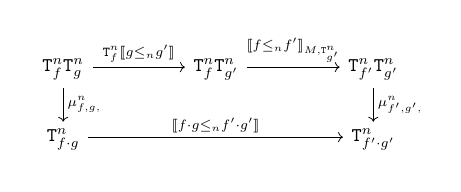
\begin{tikzpicture}[baseline= (a).base]
                    \node[scale=.7] (a) at (0,0){
                    \begin{tikzcd}
                        \Tn{f}{\Tn{g}{}} 
                        \arrow [rr, "\Tn{f}{\deno{g\subeffectn g'}
                        }"]
                        \arrow [d, "\bindn{f}{g}{}"]
                        &  &
                        \Tn{f}{\Tn{g'}{}}
                        \arrow [rr, "\db{f \subeffectn f'}_{M, \Tn{g'}{}}"]
                        & &
                         \Tn{f'}{\Tn{g'}{}} 
                         \arrow [d, "\bindn{f'}{g'}{}"]
                         \\
                        \Tn{f\dot g}{}
                        \arrow [rrrr, "\deno{f\dot g\subeffectn f'\dot g'}"]
                        & &
                         & &
                        \Tn{f'\dot g'}{}
                    \end{tikzcd}                    
                    };
            \end{tikzpicture}
            \end{minipage}
            \quad
            \begin{minipage}{.45\textwidth}
                \centering
                \scalebox{.75}{\parbox{\linewidth}{%
                \begin{align*}
                    & (\dsen{f\dot g}{f'\dot g'}_A\after\bindn{f}{g}{A})\ev \\ & = \dsez{(f\ev)\dot(g\ev)}{(f'\ev)\dot (g\ev)}_{A\ev}\after\bindz{(f\ev)}{(g\ev)}{(A\ev)}\\
                    & = \bindz{(f\ev)}{(g\ev)}{(A\ev)}\after\dsez{f\ev}{f'\ev}_{\Tz{g'\ev}{(A\ev)}}\after \Tz{f\ev}{\dsez{g\ev}{g'\ev}}_{(A\ev)}\\
                    &= \bindn{f}{g}{A}\after\dsen{f}{f'}_{\Tn{g'}{A}}\after\Tn{f}{\dsen{g}{g'}}_A
                \end{align*}
                }}
            \end{minipage}
        \end{framed}
        
    \end{framed}
    \caption{The required properties of the subeffect natural transformations can be proved component-wise from the appropriate of the subeffect natural transformation on $\set$.}
    \label{SubeffectProperties}
\end{figure}

\section{Re-indexing Functors}
\label{ReindexingFunctorProperties}
For a function $\theta: E^m \rightarrow E^n$ , the re-indexing functor $\theta\star$ is defined as follows:

\begin{align*}
    \theta\star:\quad& [E^n, \set] \rightarrow [E^m, \set]\\
    \theta\star(A)\emv=&\quad A(\theta (\emv))\\
    f:\quad& A \rightarrow B \in[E^n, \set]\\
    \theta\star(f)\emv =&\quad f(\theta(\emv)): A(\theta(\emv)\rightarrow B(\theta(\emv)))
\end{align*}

This functor preserves all the S-category properties.
These can be seen in figures \ref{PreservesCCC}-\ref{PreservesSubtypingSubeffecting}


\begin{figure}
    \centering
        \begin{framed}
            \centering\textbf{$\theta\star$ is Cartesian Closed}

            \begin{minipage}{.45\linewidth}
                \begin{align*}
                    (\theta\star(A\times B))\ev & = (A\times B)(\theta\ev)\\
                    & = (A(\theta \ev)\times B(\theta\ev))\\
                    & = (\theta\star A\times \theta\star B)\ev\\
                \end{align*}              
            \end{minipage}
            \quad
            \begin{minipage}{.45\linewidth}
                \begin{align*}
                    (\theta\star \p)\ev & = \p(\theta\ev)\\
                    & = \p \qt{Constant function}\\
                    & = \p\ev
                \end{align*}                
            \end{minipage}


            \begin{minipage}{.45\linewidth}
                \begin{align*}
                    (\theta\star \pp)\ev & = \pp(\theta\ev)\\
                    & = \pp \qt{Constant function}\\
                    & = \pp\ev
                \end{align*}                
            \end{minipage}
            \quad
            \begin{minipage}{.45\linewidth}
                \begin{align*}
                    (\theta\star\pr{f}{g})\ev & = (\pr{f}{g})(\theta\ev)\\
                    & = \pr{f(\theta\ev)}{g(\theta\ev)}\\
                    &= \pr{\theta\star f}{\theta\star g}\ev
                \end{align*}
            \end{minipage}

            \begin{minipage}{.45\linewidth}
                \begin{align*}
                    (\theta\star(A^B))\ev & = (A^B)(\theta\ev)\\
                     & = (A (\theta\ev))^{(B (\theta\ev))}\\
                     & = (\theta\star A)^{(\theta\star B)}\ev\\
                \end{align*}                
            \end{minipage}
            \quad
            \begin{minipage}{.45\linewidth}
                \begin{align*}
                (\theta\star \app)\ev & = \app(\theta\ev)\\
                & = \app \qt{Constant fn}\\
                & = \app\ev
            \end{align*}
            \end{minipage}

        \begin{minipage}{.45\linewidth}
            \begin{align*}
                (\theta\star\cur{f})\ev & = \cur{f}(\theta\ev)\\
                & = \cur{f(\theta\ev)}\\
                & = \cur{\theta\star f}
            \end{align*}             
        \end{minipage}
        \quad
        \begin{minipage}{.45\linewidth}
            \begin{align*}
                (\theta\star \1)\ev & = \1(\theta\ev)\\
                & = \1 \\
                & = \1 \ev\\
            \end{align*}
        \end{minipage}      
        
        \begin{minipage}{\linewidth}
            \begin{align*}
                (\theta\star\term{A})\ev & = \term{A}(\theta\ev)\\
                & = \term{A(\theta\ev)}\\
                & = \term{\theta\star A}\ev
            \end{align*}
        \end{minipage}        
    \end{framed}
    
    \caption{Proof of the CCC-preserving property of re-indexing functors.}
    \label{PreservesCCC}
\end{figure}

\begin{figure}
    \centering
    \begin{framed}
        \centering\textbf{$\theta\star$ Preserves Co-products}

        \begin{minipage}{.45\textwidth}
            \begin{align*}
                (\theta\star(\1 + \1))\ev & = (\1 + \1)(\theta\ev)\\
                & = (\1 + \1)\qt{Constant function}\\
                & = (\1 + \1)\ev
            \end{align*}
        \end{minipage}
        \quad
        \begin{minipage}{.45\textwidth}
            \begin{align*}
                (\theta\star\inl )\ev & = \inl(\theta\ev)\\
                & = \inl \qt{Constant Fn}\\
                & = \inl \ev
            \end{align*}
        \end{minipage}

        \begin{minipage}{.45\textwidth}
            \begin{align*}
                (\theta\star\inr )\ev & = \inr(\theta\ev)\\
                & = \inr \qt{Constant Fn}\\
                & = \inr \ev
            \end{align*}
        \end{minipage}
        \quad
        \begin{minipage}{.45\textwidth}
            \begin{align*}
                (\theta\star [f, g])\ev & = [f, g](\theta\ev)\\
                & = [f (\theta\ev), g(\theta\ev)]\\
                & = [\theta\star f, \theta\star g]\ev\\
            \end{align*}
        \end{minipage}        
    \end{framed}
    
    \caption{Proof that re-indexing functors preserve the $\1 + \1$ co-product.}
    \label{PreservesCoProduct}
\end{figure}



\begin{figure}
    \centering
    \begin{framed}
        \centering\textbf{$\theta\star$ Preserves the Graded Monad}

        \begin{minipage}{.45\textwidth}
            \begin{align*}
                (\theta\star\Tn{f}{A})\ev & = \Tn{f}{A}(\theta\ev) \\
                & = \Tz{(f(\theta\ev))}{(A(\theta\ev))}\\
                & = (\Tm{(f\after\theta)}{\theta\star A})\ev\\
            \end{align*}
        \end{minipage}
        \quad
        \begin{minipage}{.45\textwidth}
            \begin{align*}
                (\theta\star\pointn{A})\ev & = \pointn{A}(\theta\ev) \\
                & = \pointz{A(\theta\ev)}\\
                & = \pointm{\theta\star A}\ev\\
            \end{align*}
        \end{minipage}

        \begin{minipage}{.45\textwidth}
            \begin{align*}
                (\theta\star \bindn{f}{g}{A})\ev & = \bindn{f}{g}{A}(\theta\ev)\\
                & = \bindz{f(\theta\ev)}{g(\theta\ev)}{A(\theta\ev)}\\
                & = \bindm{f\after\theta}{g\after\theta}{\theta\star(A)}(\ev)
            \end{align*}
        \end{minipage}
        \quad
        \begin{minipage}{.45\textwidth}
            \begin{align*}
                (\theta\star \tstrengthn{f}{A}{B})\ev & = \tstrengthn{f}{A}{B}(\theta \ev)\\
                & = \tstrengthz{(f(\theta\ev))}{(A(\theta\ev))}{(B(\theta\ev))}\\
                & = \tstrengthm{f\after\theta}{\theta\star A}{\theta\star B}\ev\\
            \end{align*}
        \end{minipage}        
    \end{framed}
    
    \caption{Re-indexing functors preserve the graded monad structure}
    \label{GradedMonadPreserved}
\end{figure}

\begin{figure}
    \begin{framed}
        \centering\textbf{$\theta\star$ preserves Ground Subtyping and Subeffecting}

        \begin{minipage}{.45\textwidth}
            \begin{align*}
                \theta\star(\deno{A\subtypeg B})\ev  & = \deno{A\subtypeg B}(\theta\ev)\\
                & = \deno{A\subtype B} \qt{Constant Function}\\
                & = \deno{A\subtype B} \ev\\
            \end{align*}
        \end{minipage}
        \quad
        \begin{minipage}{.45\textwidth}
            \begin{align*}
                (\theta\star(\dsen{f}{g} A))\ev & = (\dsen{f}{g} A)(\theta \ev)\\
                & = (\dsen{f(\theta\ev)}{g(\theta\ev)}(A(\theta\ev)))\\
                & = (\dsem{\theta\star f}{\theta\star g} (\theta\star A)) \ev\\
            \end{align*}
        \end{minipage}
    \end{framed}
    \caption{Re-indexing functors preserve the ground subtyping and subeffecting morphisms.}
    \label{PreservesSubtypingSubeffecting}
\end{figure}


\subsection{Quantification}
We need to define $\allEn: [E^{n+1}, \set]\rightarrow[E^n, \set]$

So
\begin{align*}
    (\allEn A)\env =&\quad \Pi_{\e\in E} A(\env, \e)\\
    m:&\quad A\rightarrow B\\
    (\allEn m):&\quad \allEn A\rightarrow \allEn B\\
    (\allEn m)\env =&\Pi_{\e\in E} m(\env, \e)\\
\end{align*}

\end{document}